\documentclass[svgnames,11pt]{beamer}
\input{/home/tof/Documents/Cozy/latex-include/preambule_commun.tex}
\input{/home/tof/Documents/Cozy/latex-include/preambule_beamer.tex}
%\usepackage{pgfpages} \setbeameroption{show notes on second screen=left}
\author[]{Christophe Viroulaud}
\title{Parcours et\\structures linéaires}
\date{\framebox{\textbf{Algo 21}}}
%\logo{}
\institute{Terminale - NSI}
%DODO revoir coloration GRIS BLANC NOIR dans les schémas du BFS
\begin{document}
\begin{frame}
\titlepage
\end{frame}
\begin{frame}
    \frametitle{}

    L'algorithme de parcours en profondeur est récursif. Il est alors naturel de pouvoir l'écrire à nouveau avec une structure linéaire: la \textbf{pile}.
    \begin{framed}
        Comment implémenter les algorithmes de parcours avec des structures linéaires?
    \end{framed}

\end{frame}
\section{Rappels}
\subsection{Les structures linéaires}
\begin{frame}
    \frametitle{Rappels: Les structures linéaires}
    \begin{center}
    

        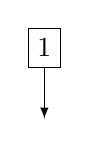
\begin{tikzpicture}[scale=0.6]
            \node[draw,minimum height=0.5cm] (s)at (0,0) {1};  
            \draw[->,>=latex] (s) -- (0,-1.5);
        \end{tikzpicture}
        \captionof{figure}{Un nœud}
    \end{center}
    \begin{activite}
    \begin{enumerate}
        \item Créer un fichier \textbf{\texttt{structures.py}}
        \item Écrire la classe \textbf{\texttt{Noeud}} et son constructeur qui, lors de l'instanciation, initialisera deux attributs:
        \begin{itemize}
            \item \textbf{\texttt{nom: int}} le nom du nœud,
            \item \textbf{\texttt{suivant: Noeud}} le successeur dans la structure.
            \item Écrire les accesseurs et les mutateurs des attributs. 
        \end{itemize}
    \end{enumerate}
    \end{activite}

\end{frame}
\begin{frame}[fragile]
    \frametitle{Correction}

\begin{center}
\begin{lstlisting}[language=Python , basicstyle=\ttfamily\small, xleftmargin=0.2em, xrightmargin=0em]
class Noeud:
    def __init__(self, nom: int, suivant: object):
        self.nom = nom
        self.suivant = suivant

    def get_nom(self) -> int:
        return self.nom

    def set_nom(self, n: int) -> None:
        self.nom = n

    def get_suivant(self) -> object:
        return self.suivant

    def set_suivant(self, s: object) -> None:
        self.suivant = s
\end{lstlisting}
\end{center} 

\end{frame}
\begin{frame}
    \frametitle{Rappels: les structures linéaires}

    \begin{center}
    

        \begin{tikzpicture}[scale=0.6]
            \foreach \v/\y in {2/8,5/6,3/4,9/2}{
            \node[draw,minimum height=0.5cm] at (0,\y) {\v};
            \draw[->,>=latex] (0,\y-.5) -- (0,\y-1.5);
            }  
            \node at (0,0) {fin};  
            \node (s) at (4,8) {sommet};
            \draw[->,>=latex] (s) -- (0.5,8);
        \end{tikzpicture}
        \captionof{figure}{Pile}
    \end{center}

\end{frame}
\begin{frame}

    \begin{activite}
    \begin{enumerate}
        \item Écrire la classe \textbf{\texttt{Pile}} et son constructeur qui initialisera l'attribut \textbf{\texttt{sommet}} à \textbf{\texttt{None}}.
        \item Écrire la méthode \textbf{\texttt{est\_vide}} qui renverra \textbf{\texttt{True}} si la pile est vide.
        \item Écrire la méthode \textbf{\texttt{empiler}} qui empilera le nœud nommé \textbf{\texttt{n: int}} passé en paramètre.
        \item Écrire la méthode \textbf{\texttt{depiler}} qui dépilera le nœud au sommet de la pile et renverra son nom ou -1 si la pile est vide.
    \end{enumerate}
    \end{activite}

\end{frame}
\begin{frame}[fragile]
    \frametitle{Correction}

\begin{center}
\begin{lstlisting}[language=Python , basicstyle=\ttfamily\small, xleftmargin=0.2em, xrightmargin=0em]
class Pile:
    def __init__(self):
        self.sommet = None

    def est_vide(self) -> bool:
        return self.sommet is None
\end{lstlisting}
\end{center} 

\end{frame}
\begin{frame}[fragile]
    \frametitle{}

\begin{center}
\begin{lstlisting}[language=Python , basicstyle=\ttfamily\small, xleftmargin=0.2em, xrightmargin=0em]
    def empiler(self, n: int) -> None:
        self.sommet = Noeud(n, self.sommet)

    def depiler(self) -> int:
        res = -1
        if not self.est_vide():
            res = self.sommet.get_nom()
            self.sommet = self.sommet.get_suivant()
        return res
\end{lstlisting}
\end{center} 

\end{frame}
\begin{frame}
    \frametitle{}

    \begin{center}
    

        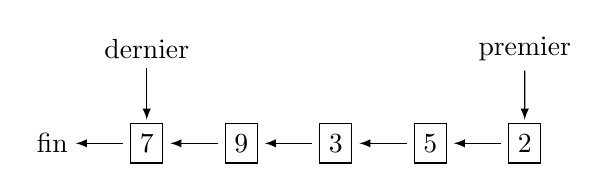
\begin{tikzpicture}[scale=0.6]
            \foreach \v/\x in {2/8,5/6,3/4,9/2}{
            \node[draw,minimum height=0.5cm] at (\x,0) {\v};
            \draw[->,>=latex] (\x-.5,0) -- (\x-1.5,0);
            }  
            \draw[->,>=latex] (-.5,0) -- (-1.5,0);
            \node at (-2,0) {fin};
            \node[draw,minimum height=0.5cm] at (0,0) {7};
            \node (p) at (8,2) {premier};
            \draw[->,>=latex] (p) -- (8,0.5);
            \node (d) at (0,2) {dernier};
            \draw[->,>=latex] (d) -- (0,0.5);
        \end{tikzpicture}
        \captionof{figure}{File}
    \end{center}

\end{frame}
\begin{frame}

    \begin{activite}
    \begin{enumerate}
        \item Écrire la classe \textbf{\texttt{File}} et son constructeur qui initialisera à \textbf{\texttt{None}} deux attributs:
        \begin{itemize}
            \item \textbf{\texttt{premier}},
            \item \textbf{\texttt{dernier}}.
        \end{itemize}
        \item Écrire la méthode \textbf{\texttt{est\_vide}} qui renverra \textbf{\texttt{True}} si la file est vide.
        \item Écrire la méthode \textbf{\texttt{enfiler}} qui enfilera le nœud nommé \textbf{\texttt{n: int}} passé en paramètre.
        \item Écrire la méthode \textbf{\texttt{defiler}} qui défilera le nœud en première place de la file et renverra son nom ou -1 si la file est vide.
    \end{enumerate}
    \end{activite}

\end{frame}
\begin{frame}[fragile]
    \frametitle{Correction}
\begin{center}
\begin{lstlisting}[language=Python , basicstyle=\ttfamily\small, xleftmargin=2em, xrightmargin=2em]
class File:
    def __init__(self):
        self.premier = None
        self.dernier = None

    def est_vide(self) -> bool:
        return self.premier is None

    
\end{lstlisting}
\end{center}
    

\end{frame}
\begin{frame}[fragile]
    \frametitle{}

\begin{center}
\begin{lstlisting}[language=Python , basicstyle=\ttfamily\small, xleftmargin=0.2em, xrightmargin=-1em]
    def enfiler(self, n: int) -> None:
        nouveau = Noeud(n, None)
        if self.est_vide():
            self.premier = nouveau
        else:
            self.dernier.set_suivant(nouveau)
        self.dernier = nouveau

    def defiler(self) -> int:
        res = -1
        if not self.est_vide():
            res = self.premier.get_nom()
            self.premier = self.premier.get_suivant()
        return res
\end{lstlisting}
\end{center} 

\end{frame}
\subsection{Représentation d'un graphe en mémoire}
\begin{frame}
    \frametitle{Représentation d'un graphe en mémoire}

    \begin{center}
        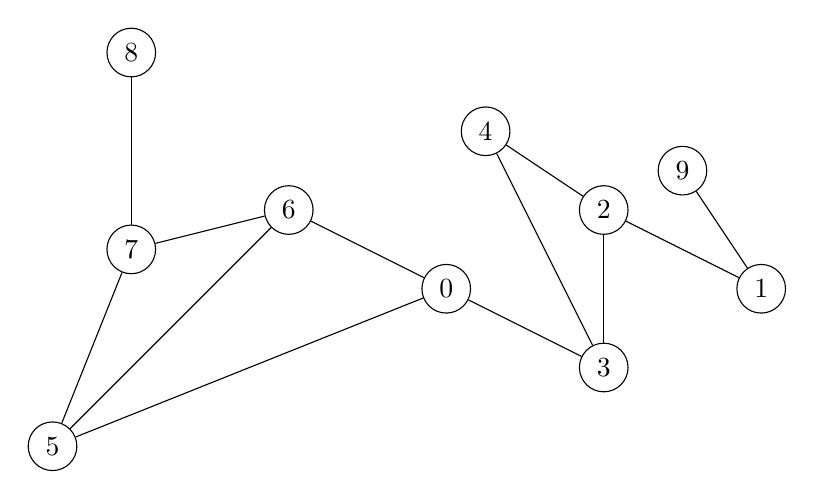
\begin{tikzpicture}
            \node[draw,circle] (0)at(0,0) {0};
            \node[draw,circle] (1)at(4,0) {1};
            \node[draw,circle] (2)at(2,1) {2};
            \node[draw,circle] (3)at(2,-1) {3};
            \node[draw,circle] (4)at(0.5,2) {4};
            \node[draw,circle] (5)at(-5,-2) {5};
            \node[draw,circle] (6)at(-2,1) {6};
            \node[draw,circle] (7)at(-4,0.5) {7};
            \node[draw,circle] (8)at(-4,3) {8};
            \node[draw,circle] (9)at(3,1.5) {9};

            \draw[-,>=latex] (1) -- (2);
            \draw[-,>=latex] (9) -- (1);
            \draw[-,>=latex] (4) -- (2);
            \draw[-,>=latex] (7) -- (8);
            \draw[-,>=latex] (5) -- (6);
            \draw[-,>=latex] (6) -- (7);
            \draw[-,>=latex] (7) -- (5);
            \draw[-,>=latex] (6) -- (0);
            \draw[-,>=latex] (0) -- (3);
            \draw[-,>=latex] (5) -- (0);
            \draw[-,>=latex] (3) -- (2);
            \draw[-,>=latex] (3) -- (4);

        \end{tikzpicture}
    \end{center}
\begin{activite}
\begin{enumerate}
    \item Créer le fichier \textbf{\texttt{parcours.py}}
    \item Écrire la liste d'adjacence du graphe.
\end{enumerate}
\end{activite}
\end{frame}
\begin{frame}[fragile]
    \frametitle{Correction}

\begin{center}
\begin{lstlisting}[language=Python , basicstyle=\ttfamily\small, xleftmargin=2em, xrightmargin=2em]
graphe = [
    [3, 5, 6],
    [2, 9],
    [1, 3, 4],
    [0, 2, 4],
    [2, 3],
    [0, 6, 7],
    [0, 5, 7],
    [5, 6, 8],
    [7],
    [1]
]
\end{lstlisting}
\end{center}

\end{frame}
\section{Parcours en profondeur}
\begin{frame}
    \frametitle{Parcours en profondeur}

\begin{aretenir}[]
Lors d'un parcours en profondeur on repart du nœud en cours de visite pour continuer le parcours. On utilise alors une \textbf{pile} pour l'implémenter.
\end{aretenir}

\end{frame}
\begin{frame}
    \frametitle{}
\begin{activite}
\begin{enumerate}
    \item Écrire la fonction \textbf{\texttt{dfs(graphe: list) $\rightarrow$ list}} qui effectue un parcours en profondeur en utilisant une pile. La fonction renverra la liste ordonnée des sommets parcourus.
    \item Écrire la fonction \textbf{\texttt{dfs\_aretes(graphe: list) $\rightarrow$ list}} qui renvoie les liste ordonnée des arêtes parcourues. La fonction colorera les sommets en:
    \begin{itemize}
        \item \textbf{\texttt{BLANC}} au départ,
        \item \textbf{\texttt{GRIS}} lors de l'empilement,
        \item \textbf{\texttt{NOIR}} quand son parcours est terminé.
    \end{itemize}
\end{enumerate}
\end{activite}
    

\end{frame}
\begin{frame}[fragile]
    \frametitle{Correction}
\begin{center}
\begin{lstlisting}[language=Python , basicstyle=\ttfamily\small, xleftmargin=2em, xrightmargin=2em]
def dfs(graphe: list) -> list:
    parcours = []
    p = Pile()
    p.empiler(0)
    while not p.est_vide():
        en_cours = p.depiler()
        if en_cours not in parcours:
            parcours.append(en_cours)

            for voisin in graphe[en_cours]:
                p.empiler(voisin)
    return parcours
\end{lstlisting}
\begin{lstlisting}[language=Python , basicstyle=\ttfamily\small, xleftmargin=2em, xrightmargin=2em]
>>> dfs(graphe)
[0, 6, 7, 8, 5, 3, 4, 2, 1, 9]
\end{lstlisting}
\captionof{code}{Appel de la fonction}
\label{CODE}
\end{center}
    

\end{frame}
\begin{frame}[fragile]
    \frametitle{Correction}
\begin{center}
\begin{lstlisting}[language=Python , basicstyle=\ttfamily\small, xleftmargin=0.2em, xrightmargin=-1em]
def dfs_aretes(graphe: list) -> list:
    parcours = []
    etats = [BLANC for _ in range(len(graphe))]
    p = Pile()
    p.empiler(0)
    while not p.est_vide():
        en_cours = p.depiler()
        for voisin in graphe[en_cours]:
            if etats[voisin] == BLANC:
                etats[voisin] = GRIS
                p.empiler(voisin)
            # stockage arête parcourue
            parcours.append((en_cours, voisin))
                
        etats[en_cours] = NOIR
    return parcours
\end{lstlisting}

\end{center}
    

\end{frame}
\begin{frame}[fragile]
    \frametitle{}
    \begin{center}
        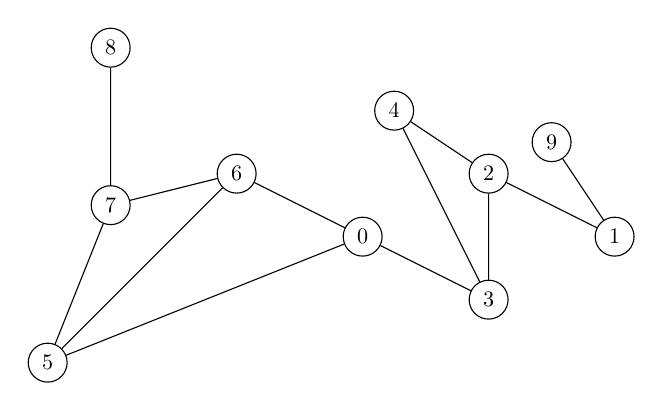
\begin{tikzpicture}[scale=0.8, transform shape]
            \node[draw,circle] (0)at(0,0) {0};
            \node[draw,circle] (1)at(4,0) {1};
            \node[draw,circle] (2)at(2,1) {2};
            \node[draw,circle] (3)at(2,-1) {3};
            \node[draw,circle] (4)at(0.5,2) {4};
            \node[draw,circle] (5)at(-5,-2) {5};
            \node[draw,circle] (6)at(-2,1) {6};
            \node[draw,circle] (7)at(-4,0.5) {7};
            \node[draw,circle] (8)at(-4,3) {8};
            \node[draw,circle] (9)at(3,1.5) {9};

            \draw[-,>=latex] (1) -- (2);
            \draw[-,>=latex] (9) -- (1);
            \draw[-,>=latex] (4) -- (2);
            \draw[-,>=latex] (7) -- (8);
            \draw[-,>=latex] (5) -- (6);
            \draw[-,>=latex] (6) -- (7);
            \draw[-,>=latex] (7) -- (5);
            \draw[-,>=latex] (6) -- (0);
            \draw[-,>=latex] (0) -- (3);
            \draw[-,>=latex] (5) -- (0);
            \draw[-,>=latex] (3) -- (2);
            \draw[-,>=latex] (3) -- (4);

        \end{tikzpicture}
    \end{center}
\begin{center}
\begin{lstlisting}[language=Python , basicstyle=\ttfamily\small, xleftmargin=0.2em, xrightmargin=0.5em]
>>> dfs_aretes(graphe)
[(0, 3), (0, 5), (0, 6), (6, 0), (6, 5), (6, 7), (7, 5), (7, 6), (7, 8), (8, 7), (5, 0), (5, 6), (5, 7), (3, 0), (3, 2), (3, 4), (4, 2), (4, 3), (2, 1), (2, 3), (2, 4), (1, 2), (1, 9), (9, 1)]
\end{lstlisting}
\captionof{code}{\centering Chaque sommet n'est empilé qu'une seule fois. Chaque arête est parcourue deux fois (graphe non orienté).}
\label{CODE}
\end{center}
\end{frame}
\begin{frame}[fragile]
    \frametitle{}
    \begin{center}
        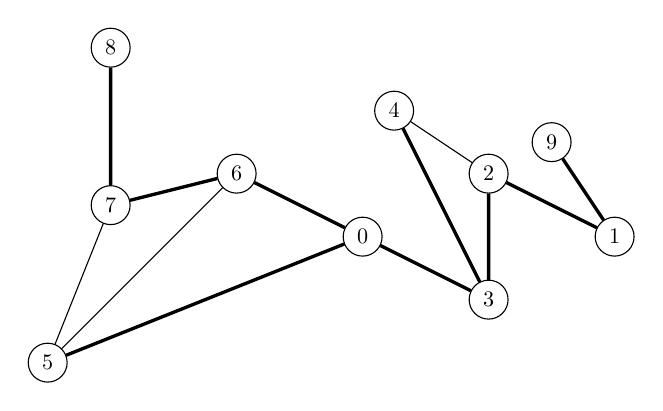
\begin{tikzpicture}[scale=0.8, transform shape]
            \node[draw,circle] (0)at(0,0) {0};
            \node[draw,circle] (1)at(4,0) {1};
            \node[draw,circle] (2)at(2,1) {2};
            \node[draw,circle] (3)at(2,-1) {3};
            \node[draw,circle] (4)at(0.5,2) {4};
            \node[draw,circle] (5)at(-5,-2) {5};
            \node[draw,circle] (6)at(-2,1) {6};
            \node[draw,circle] (7)at(-4,0.5) {7};
            \node[draw,circle] (8)at(-4,3) {8};
            \node[draw,circle] (9)at(3,1.5) {9};

            \draw[-,>=latex,very thick] (1) -- (2);
            \draw[-,>=latex,very thick] (9) -- (1);
            \draw[-,>=latex] (4) -- (2);
            \draw[-,>=latex,very thick] (7) -- (8);
            \draw[-,>=latex] (5) -- (6);
            \draw[-,>=latex,very thick] (6) -- (7);
            \draw[-,>=latex] (7) -- (5);
            \draw[-,>=latex,very thick] (6) -- (0);
            \draw[-,>=latex,very thick] (0) -- (3);
            \draw[-,>=latex,very thick] (5) -- (0);
            \draw[-,>=latex,very thick] (3) -- (2);
            \draw[-,>=latex,very thick] (3) -- (4);

        \end{tikzpicture}
    \end{center}
\begin{center}
\begin{lstlisting}[language=Python , basicstyle=\ttfamily\small, xleftmargin=2em, xrightmargin=2em]
[(0, 3), (0, 5), (0, 6), (6, 7), (7, 8), (3, 2), (3, 4), (2, 1), (1, 9)]
\end{lstlisting}
\end{center}   
\begin{aretenir}[Observation]
Si on stocke les arêtes seulement quand on empile les voisins, elles ne sont pas toutes visitées.
\end{aretenir}
\end{frame}
\section{Parcours en largeur}
\subsection{Principe}
\begin{frame}
    \frametitle{Parcours en largeur - Principe}

    
\begin{aretenir}[]
Le parcours en largeur visite tous les sommets au rang \textbf{\texttt{n}} avant ceux au rang \textbf{\texttt{n+1}}. On utilise une \textbf{file} pour l'implémenter.
\end{aretenir}
\end{frame}
\begin{frame}
    \frametitle{}

    \begin{center}
        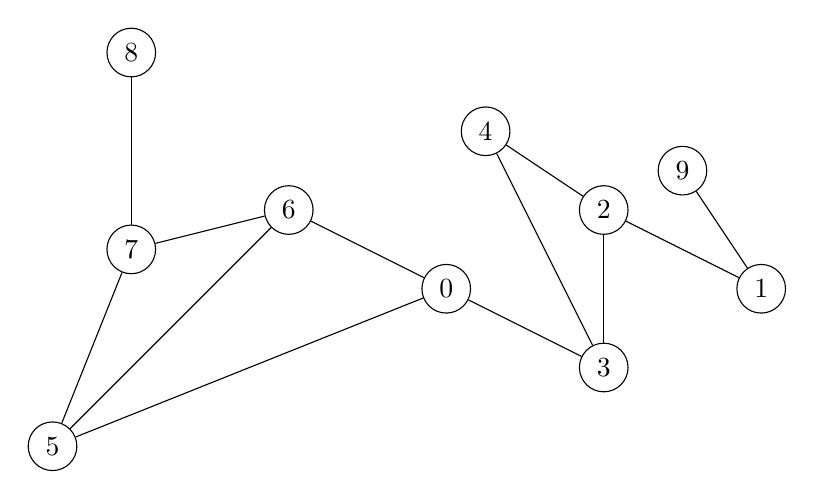
\begin{tikzpicture}
            \node[draw,circle] (0)at(0,0) {0};
            \node[draw,circle] (1)at(4,0) {1};
            \node[draw,circle] (2)at(2,1) {2};
            \node[draw,circle] (3)at(2,-1) {3};
            \node[draw,circle] (4)at(0.5,2) {4};
            \node[draw,circle] (5)at(-5,-2) {5};
            \node[draw,circle] (6)at(-2,1) {6};
            \node[draw,circle] (7)at(-4,0.5) {7};
            \node[draw,circle] (8)at(-4,3) {8};
            \node[draw,circle] (9)at(3,1.5) {9};

            \draw[-,>=latex] (1) -- (2);
            \draw[-,>=latex] (9) -- (1);
            \draw[-,>=latex] (4) -- (2);
            \draw[-,>=latex] (7) -- (8);
            \draw[-,>=latex] (5) -- (6);
            \draw[-,>=latex] (6) -- (7);
            \draw[-,>=latex] (7) -- (5);
            \draw[-,>=latex] (6) -- (0);
            \draw[-,>=latex] (0) -- (3);
            \draw[-,>=latex] (5) -- (0);
            \draw[-,>=latex] (3) -- (2);
            \draw[-,>=latex] (3) -- (4);

        \end{tikzpicture}
        \captionof{figure}{Départ}
    \end{center}
\begin{center}
    File: \textbf{\texttt{0}}
\end{center}
\end{frame}
\begin{frame}
    \frametitle{}

    \begin{center}
        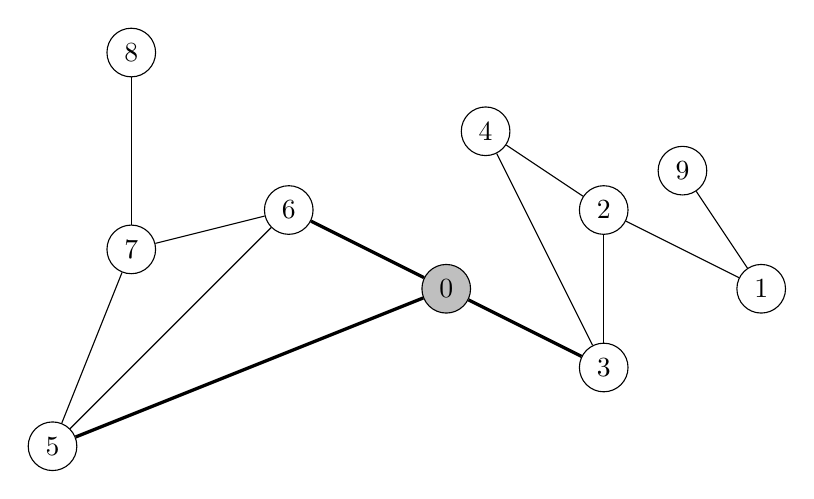
\begin{tikzpicture}
            \node[draw,circle, fill=gray!50] (0)at(0,0) {0};
            \node[draw,circle] (1)at(4,0) {1};
            \node[draw,circle] (2)at(2,1) {2};
            \node[draw,circle] (3)at(2,-1) {3};
            \node[draw,circle] (4)at(0.5,2) {4};
            \node[draw,circle] (5)at(-5,-2) {5};
            \node[draw,circle] (6)at(-2,1) {6};
            \node[draw,circle] (7)at(-4,0.5) {7};
            \node[draw,circle] (8)at(-4,3) {8};
            \node[draw,circle] (9)at(3,1.5) {9};

            \draw[-,>=latex] (1) -- (2);
            \draw[-,>=latex] (9) -- (1);
            \draw[-,>=latex] (4) -- (2);
            \draw[-,>=latex] (7) -- (8);
            \draw[-,>=latex] (5) -- (6);
            \draw[-,>=latex] (6) -- (7);
            \draw[-,>=latex] (7) -- (5);
            \draw[-,>=latex, very thick] (6) -- (0);
            \draw[-,>=latex, very thick] (0) -- (3);
            \draw[-,>=latex, very thick] (5) -- (0);
            \draw[-,>=latex] (3) -- (2);
            \draw[-,>=latex] (3) -- (4);

        \end{tikzpicture}
        \captionof{figure}{On enfile les voisins à distance 1.}
    \end{center}
\begin{center}
    File: \textbf{\texttt{6}} $\rightarrow$ \textbf{\texttt{5}} $\rightarrow$ \textbf{\texttt{3}}
\end{center}
\end{frame}
\begin{frame}
    \frametitle{}

    \begin{center}
        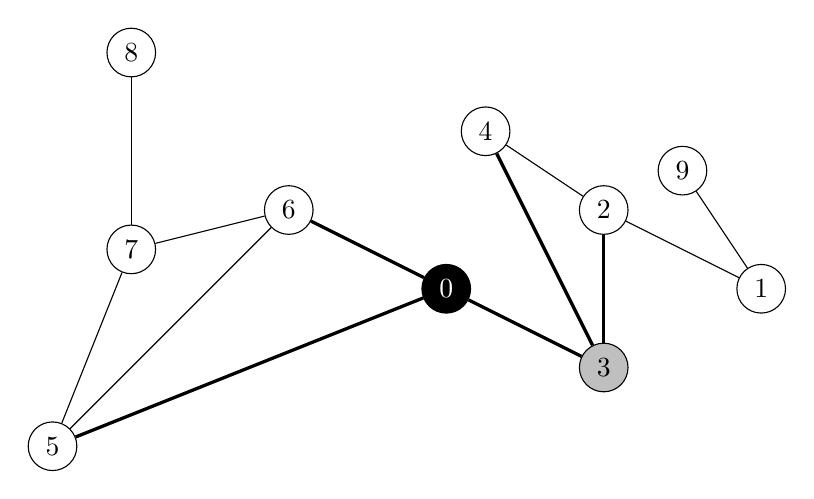
\begin{tikzpicture}
            \node[draw,circle, fill=black, text=white] (0)at(0,0) {0};
            \node[draw,circle] (1)at(4,0) {1};
            \node[draw,circle] (2)at(2,1) {2};
            \node[draw,circle, fill=gray!50] (3)at(2,-1) {3};
            \node[draw,circle] (4)at(0.5,2) {4};
            \node[draw,circle] (5)at(-5,-2) {5};
            \node[draw,circle] (6)at(-2,1) {6};
            \node[draw,circle] (7)at(-4,0.5) {7};
            \node[draw,circle] (8)at(-4,3) {8};
            \node[draw,circle] (9)at(3,1.5) {9};

            \draw[-,>=latex] (1) -- (2);
            \draw[-,>=latex] (9) -- (1);
            \draw[-,>=latex] (4) -- (2);
            \draw[-,>=latex] (7) -- (8);
            \draw[-,>=latex] (5) -- (6);
            \draw[-,>=latex] (6) -- (7);
            \draw[-,>=latex] (7) -- (5);
            \draw[-,>=latex, very thick] (6) -- (0);
            \draw[-,>=latex, very thick] (0) -- (3);
            \draw[-,>=latex, very thick] (5) -- (0);
            \draw[-,>=latex, very thick] (3) -- (2);
            \draw[-,>=latex, very thick] (3) -- (4);

        \end{tikzpicture}
        \captionof{figure}{On enfile les voisins à distance 2.}
    \end{center}
\begin{center}
    File: \textbf{\texttt{4}} $\rightarrow$ \textbf{\texttt{2}} $\rightarrow$ \textbf{\texttt{6}} $\rightarrow$ \textbf{\texttt{5}}
\end{center}
\end{frame}
\begin{frame}
    \frametitle{}

    \begin{center}
        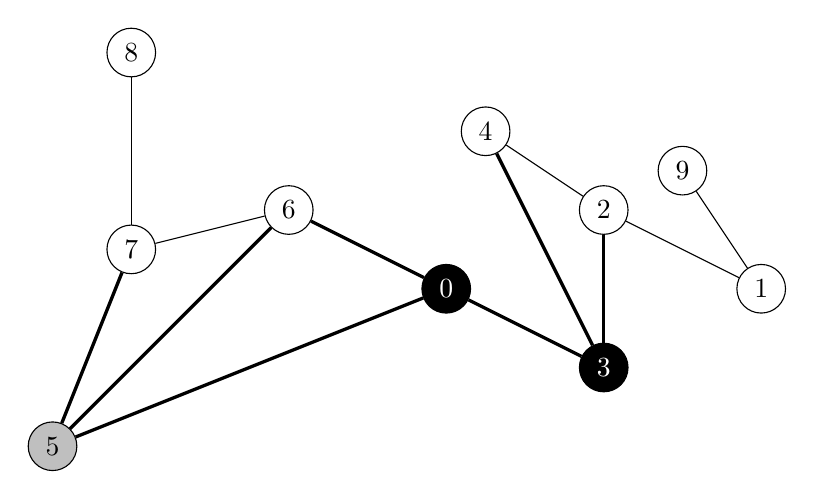
\begin{tikzpicture}
            \node[draw,circle, fill=black, text=white] (0)at(0,0) {0};
            \node[draw,circle] (1)at(4,0) {1};
            \node[draw,circle] (2)at(2,1) {2};
            \node[draw,circle, fill=black, text=white] (3)at(2,-1) {3};
            \node[draw,circle] (4)at(0.5,2) {4};
            \node[draw,circle, fill=gray!50] (5)at(-5,-2) {5};
            \node[draw,circle] (6)at(-2,1) {6};
            \node[draw,circle] (7)at(-4,0.5) {7};
            \node[draw,circle] (8)at(-4,3) {8};
            \node[draw,circle] (9)at(3,1.5) {9};

            \draw[-,>=latex] (1) -- (2);
            \draw[-,>=latex] (9) -- (1);
            \draw[-,>=latex] (4) -- (2);
            \draw[-,>=latex] (7) -- (8);
            \draw[-,>=latex, very thick] (5) -- (6);
            \draw[-,>=latex] (6) -- (7);
            \draw[-,>=latex, very thick] (7) -- (5);
            \draw[-,>=latex, very thick] (6) -- (0);
            \draw[-,>=latex, very thick] (0) -- (3);
            \draw[-,>=latex, very thick] (5) -- (0);
            \draw[-,>=latex, very thick] (3) -- (2);
            \draw[-,>=latex, very thick] (3) -- (4);

        \end{tikzpicture}
        \captionof{figure}{On enfile les voisins à distance 2.}
    \end{center}
\begin{center}
    File: \textbf{\texttt{7}} $\rightarrow$ \textbf{\texttt{4}} $\rightarrow$ \textbf{\texttt{2}} $\rightarrow$ \textbf{\texttt{6}} 
\end{center}
\end{frame}
\begin{frame}
    \frametitle{}

    \begin{center}
        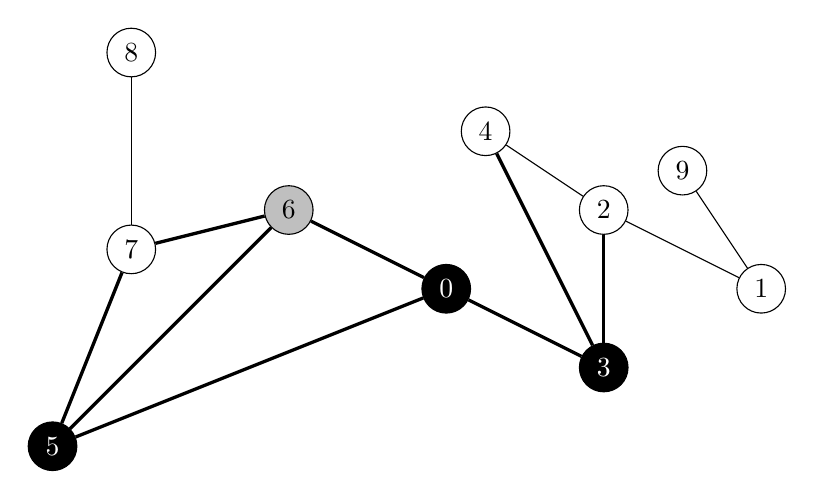
\begin{tikzpicture}
            \node[draw,circle, fill=black, text=white] (0)at(0,0) {0};
            \node[draw,circle] (1)at(4,0) {1};
            \node[draw,circle] (2)at(2,1) {2};
            \node[draw,circle, fill=black, text=white] (3)at(2,-1) {3};
            \node[draw,circle] (4)at(0.5,2) {4};
            \node[draw,circle, fill=black, text=white] (5)at(-5,-2) {5};
            \node[draw,circle, fill=gray!50] (6)at(-2,1) {6};
            \node[draw,circle] (7)at(-4,0.5) {7};
            \node[draw,circle] (8)at(-4,3) {8};
            \node[draw,circle] (9)at(3,1.5) {9};

            \draw[-,>=latex] (1) -- (2);
            \draw[-,>=latex] (9) -- (1);
            \draw[-,>=latex] (4) -- (2);
            \draw[-,>=latex] (7) -- (8);
            \draw[-,>=latex, very thick] (5) -- (6);
            \draw[-,>=latex, very thick] (6) -- (7);
            \draw[-,>=latex, very thick] (7) -- (5);
            \draw[-,>=latex, very thick] (6) -- (0);
            \draw[-,>=latex, very thick] (0) -- (3);
            \draw[-,>=latex, very thick] (5) -- (0);
            \draw[-,>=latex, very thick] (3) -- (2);
            \draw[-,>=latex, very thick] (3) -- (4);

        \end{tikzpicture}
        \captionof{figure}{On enfile les voisins à distance 2: pas de nouveau sommet pour \textbf{\texttt{6}}.}
    \end{center}
\begin{center}
    File: \textbf{\texttt{7}} $\rightarrow$ \textbf{\texttt{4}} $\rightarrow$ \textbf{\texttt{2}}
\end{center}
\end{frame}

\begin{frame}
    \frametitle{}

    \begin{center}
        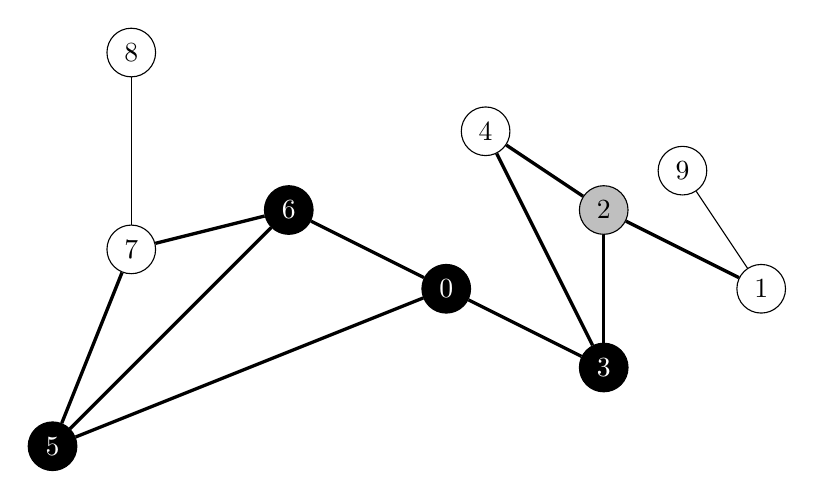
\begin{tikzpicture}
            \node[draw,circle, fill=black, text=white] (0)at(0,0) {0};
            \node[draw,circle] (1)at(4,0) {1};
            \node[draw,circle, fill=gray!50] (2)at(2,1) {2};
            \node[draw,circle, fill=black, text=white] (3)at(2,-1) {3};
            \node[draw,circle] (4)at(0.5,2) {4};
            \node[draw,circle, fill=black, text=white] (5)at(-5,-2) {5};
            \node[draw,circle, fill=black, text=white] (6)at(-2,1) {6};
            \node[draw,circle] (7)at(-4,0.5) {7};
            \node[draw,circle] (8)at(-4,3) {8};
            \node[draw,circle] (9)at(3,1.5) {9};

            \draw[-,>=latex, very thick] (1) -- (2);
            \draw[-,>=latex] (9) -- (1);
            \draw[-,>=latex, very thick] (4) -- (2);
            \draw[-,>=latex] (7) -- (8);
            \draw[-,>=latex, very thick] (5) -- (6);
            \draw[-,>=latex, very thick] (6) -- (7);
            \draw[-,>=latex, very thick] (7) -- (5);
            \draw[-,>=latex, very thick] (6) -- (0);
            \draw[-,>=latex, very thick] (0) -- (3);
            \draw[-,>=latex, very thick] (5) -- (0);
            \draw[-,>=latex, very thick] (3) -- (2);
            \draw[-,>=latex, very thick] (3) -- (4);

        \end{tikzpicture}
        \captionof{figure}{On enfile les voisins à distance 3.}
    \end{center}
\begin{center}
    File: \textbf{\texttt{1}} $\rightarrow$ \textbf{\texttt{7}} $\rightarrow$ \textbf{\texttt{4}}
\end{center}
\end{frame}

\begin{frame}
    \frametitle{}

    \begin{center}
        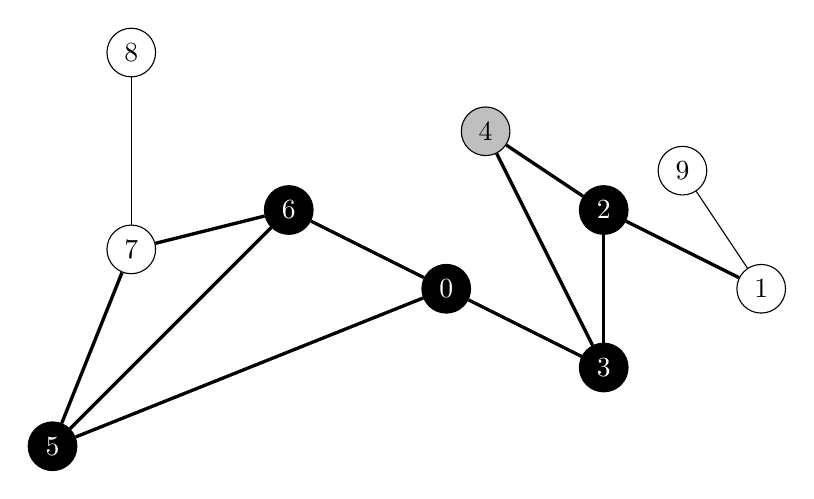
\begin{tikzpicture}
            \node[draw,circle, fill=black, text=white] (0)at(0,0) {0};
            \node[draw,circle] (1)at(4,0) {1};
            \node[draw,circle, fill=black, text=white] (2)at(2,1) {2};
            \node[draw,circle, fill=black, text=white] (3)at(2,-1) {3};
            \node[draw,circle,fill=gray!50] (4)at(0.5,2) {4};
            \node[draw,circle, fill=black, text=white] (5)at(-5,-2) {5};
            \node[draw,circle, fill=black, text=white] (6)at(-2,1) {6};
            \node[draw,circle] (7)at(-4,0.5) {7};
            \node[draw,circle] (8)at(-4,3) {8};
            \node[draw,circle] (9)at(3,1.5) {9};

            \draw[-,>=latex, very thick] (1) -- (2);
            \draw[-,>=latex] (9) -- (1);
            \draw[-,>=latex, very thick] (4) -- (2);
            \draw[-,>=latex] (7) -- (8);
            \draw[-,>=latex, very thick] (5) -- (6);
            \draw[-,>=latex, very thick] (6) -- (7);
            \draw[-,>=latex, very thick] (7) -- (5);
            \draw[-,>=latex, very thick] (6) -- (0);
            \draw[-,>=latex, very thick] (0) -- (3);
            \draw[-,>=latex, very thick] (5) -- (0);
            \draw[-,>=latex, very thick] (3) -- (2);
            \draw[-,>=latex, very thick] (3) -- (4);

        \end{tikzpicture}
        \captionof{figure}{On enfile les voisins à distance 3: pas de nouveau sommet pour 4.}
    \end{center}
\begin{center}
    File: \textbf{\texttt{1}} $\rightarrow$ \textbf{\texttt{7}} 
\end{center}
\end{frame}
\begin{frame}
    \frametitle{}

    \begin{center}
        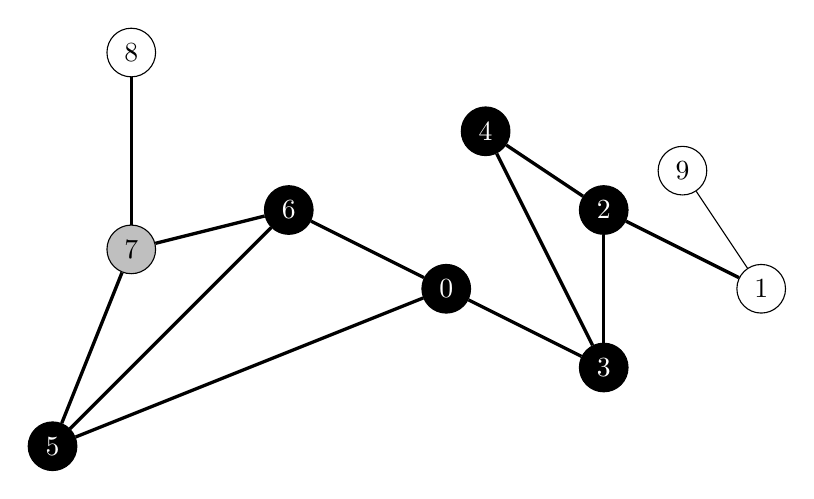
\begin{tikzpicture}
            \node[draw,circle, fill=black, text=white] (0)at(0,0) {0};
            \node[draw,circle] (1)at(4,0) {1};
            \node[draw,circle, fill=black, text=white] (2)at(2,1) {2};
            \node[draw,circle, fill=black, text=white] (3)at(2,-1) {3};
            \node[draw,circle, fill=black, text=white] (4)at(0.5,2) {4};
            \node[draw,circle, fill=black, text=white] (5)at(-5,-2) {5};
            \node[draw,circle, fill=black, text=white] (6)at(-2,1) {6};
            \node[draw,circle, fill=gray!50] (7)at(-4,0.5) {7};
            \node[draw,circle] (8)at(-4,3) {8};
            \node[draw,circle] (9)at(3,1.5) {9};

            \draw[-,>=latex, very thick] (1) -- (2);
            \draw[-,>=latex] (9) -- (1);
            \draw[-,>=latex, very thick] (4) -- (2);
            \draw[-,>=latex, very thick] (7) -- (8);
            \draw[-,>=latex, very thick] (5) -- (6);
            \draw[-,>=latex, very thick] (6) -- (7);
            \draw[-,>=latex, very thick] (7) -- (5);
            \draw[-,>=latex, very thick] (6) -- (0);
            \draw[-,>=latex, very thick] (0) -- (3);
            \draw[-,>=latex, very thick] (5) -- (0);
            \draw[-,>=latex, very thick] (3) -- (2);
            \draw[-,>=latex, very thick] (3) -- (4);

        \end{tikzpicture}
        \captionof{figure}{On enfile les voisins à distance 3.}
    \end{center}
\begin{center}
    File: \textbf{\texttt{8}} $\rightarrow$ \textbf{\texttt{1}}
\end{center}
\end{frame}
\begin{frame}
    \frametitle{}

    \begin{center}
        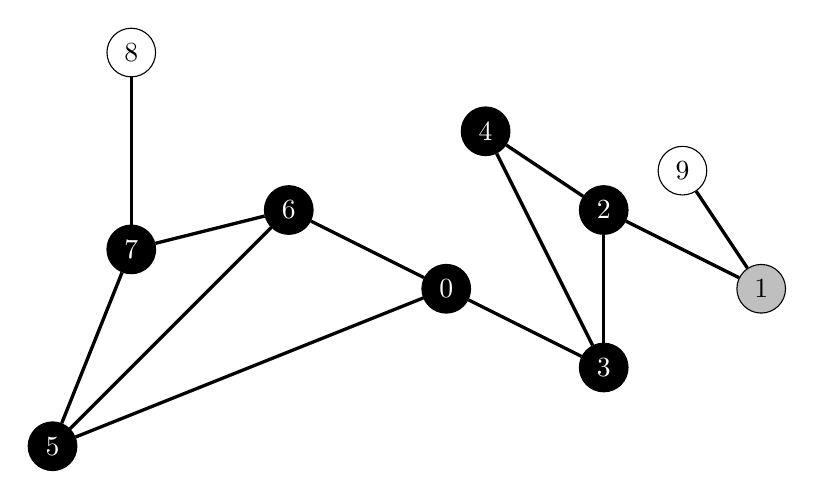
\begin{tikzpicture}
            \node[draw,circle, fill=black, text=white] (0)at(0,0) {0};
            \node[draw,circle, fill=gray!50] (1)at(4,0) {1};
            \node[draw,circle, fill=black, text=white] (2)at(2,1) {2};
            \node[draw,circle, fill=black, text=white] (3)at(2,-1) {3};
            \node[draw,circle, fill=black, text=white] (4)at(0.5,2) {4};
            \node[draw,circle, fill=black, text=white] (5)at(-5,-2) {5};
            \node[draw,circle, fill=black, text=white] (6)at(-2,1) {6};
            \node[draw,circle, fill=black, text=white] (7)at(-4,0.5) {7};
            \node[draw,circle] (8)at(-4,3) {8};
            \node[draw,circle] (9)at(3,1.5) {9};

            \draw[-,>=latex, very thick] (1) -- (2);
            \draw[-,>=latex, very thick] (9) -- (1);
            \draw[-,>=latex, very thick] (4) -- (2);
            \draw[-,>=latex, very thick] (7) -- (8);
            \draw[-,>=latex, very thick] (5) -- (6);
            \draw[-,>=latex, very thick] (6) -- (7);
            \draw[-,>=latex, very thick] (7) -- (5);
            \draw[-,>=latex, very thick] (6) -- (0);
            \draw[-,>=latex, very thick] (0) -- (3);
            \draw[-,>=latex, very thick] (5) -- (0);
            \draw[-,>=latex, very thick] (3) -- (2);
            \draw[-,>=latex, very thick] (3) -- (4);

        \end{tikzpicture}
        \captionof{figure}{On enfile les voisins à distance 4.}
    \end{center}
\begin{center}
    File: \textbf{\texttt{9}} $\rightarrow$ \textbf{\texttt{8}} 
\end{center}
\end{frame}
\begin{frame}
    \frametitle{}

    \begin{center}
        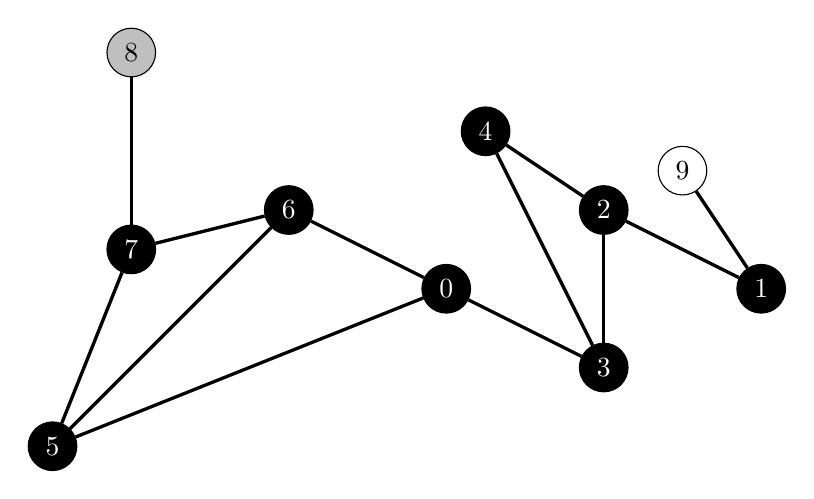
\begin{tikzpicture}
            \node[draw,circle, fill=black, text=white] (0)at(0,0) {0};
            \node[draw,circle, fill=black, text=white] (1)at(4,0) {1};
            \node[draw,circle, fill=black, text=white] (2)at(2,1) {2};
            \node[draw,circle, fill=black, text=white] (3)at(2,-1) {3};
            \node[draw,circle, fill=black, text=white] (4)at(0.5,2) {4};
            \node[draw,circle, fill=black, text=white] (5)at(-5,-2) {5};
            \node[draw,circle, fill=black, text=white] (6)at(-2,1) {6};
            \node[draw,circle, fill=black, text=white] (7)at(-4,0.5) {7};
            \node[draw,circle, fill=gray!50] (8)at(-4,3) {8};
            \node[draw,circle] (9)at(3,1.5) {9};

            \draw[-,>=latex, very thick] (1) -- (2);
            \draw[-,>=latex, very thick] (9) -- (1);
            \draw[-,>=latex, very thick] (4) -- (2);
            \draw[-,>=latex, very thick] (7) -- (8);
            \draw[-,>=latex, very thick] (5) -- (6);
            \draw[-,>=latex, very thick] (6) -- (7);
            \draw[-,>=latex, very thick] (7) -- (5);
            \draw[-,>=latex, very thick] (6) -- (0);
            \draw[-,>=latex, very thick] (0) -- (3);
            \draw[-,>=latex, very thick] (5) -- (0);
            \draw[-,>=latex, very thick] (3) -- (2);
            \draw[-,>=latex, very thick] (3) -- (4);

        \end{tikzpicture}
        \captionof{figure}{On enfile les voisins à distance 4: pas de nouveau sommet pour 8.}
    \end{center}
\begin{center}
    File: \textbf{\texttt{9}}
\end{center}
\end{frame}
\begin{frame}
    \frametitle{}

    \begin{center}
        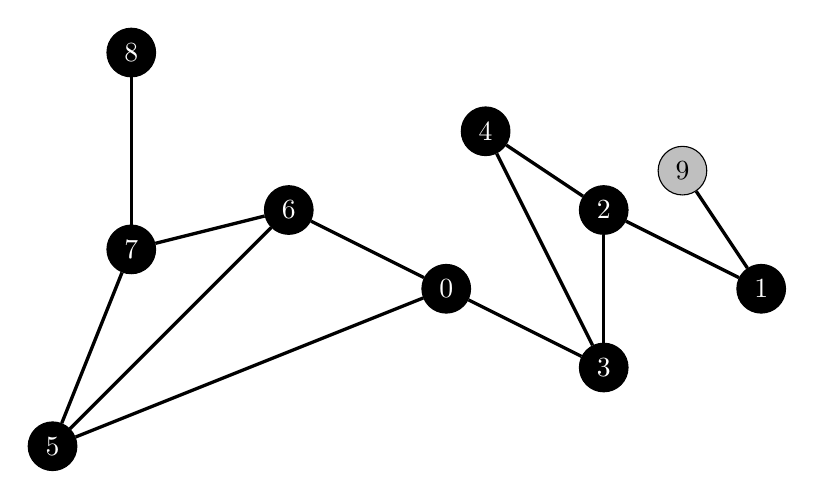
\begin{tikzpicture}
            \node[draw,circle, fill=black, text=white] (0)at(0,0) {0};
            \node[draw,circle, fill=black, text=white] (1)at(4,0) {1};
            \node[draw,circle, fill=black, text=white] (2)at(2,1) {2};
            \node[draw,circle, fill=black, text=white] (3)at(2,-1) {3};
            \node[draw,circle, fill=black, text=white] (4)at(0.5,2) {4};
            \node[draw,circle, fill=black, text=white] (5)at(-5,-2) {5};
            \node[draw,circle, fill=black, text=white] (6)at(-2,1) {6};
            \node[draw,circle, fill=black, text=white] (7)at(-4,0.5) {7};
            \node[draw,circle, fill=black, text=white] (8)at(-4,3) {8};
            \node[draw,circle, fill=gray!50] (9)at(3,1.5) {9};

            \draw[-,>=latex, very thick] (1) -- (2);
            \draw[-,>=latex, very thick] (9) -- (1);
            \draw[-,>=latex, very thick] (4) -- (2);
            \draw[-,>=latex, very thick] (7) -- (8);
            \draw[-,>=latex, very thick] (5) -- (6);
            \draw[-,>=latex, very thick] (6) -- (7);
            \draw[-,>=latex, very thick] (7) -- (5);
            \draw[-,>=latex, very thick] (6) -- (0);
            \draw[-,>=latex, very thick] (0) -- (3);
            \draw[-,>=latex, very thick] (5) -- (0);
            \draw[-,>=latex, very thick] (3) -- (2);
            \draw[-,>=latex, very thick] (3) -- (4);

        \end{tikzpicture}
        \captionof{figure}{Pas de sommet à distance 5.}
    \end{center}
\begin{center}
    File: 
\end{center}
\end{frame}
\begin{frame}
    \frametitle{}

    \begin{center}
        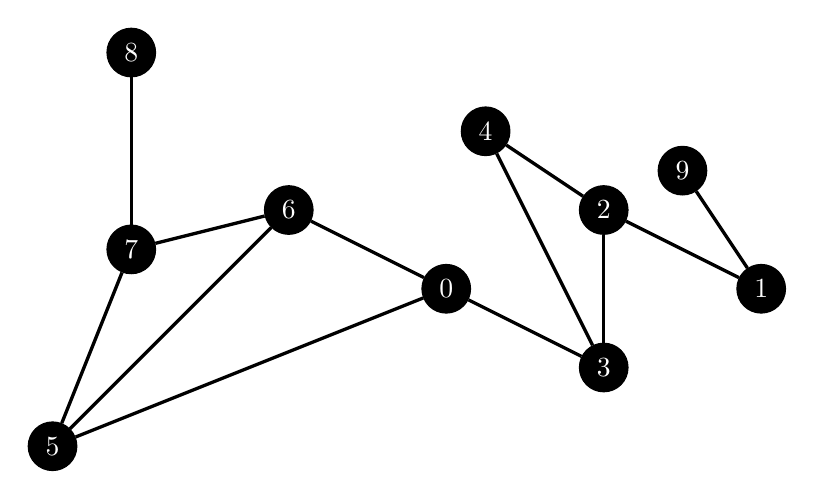
\begin{tikzpicture}
            \node[draw,circle, fill=black, text=white] (0)at(0,0) {0};
            \node[draw,circle, fill=black, text=white] (1)at(4,0) {1};
            \node[draw,circle, fill=black, text=white] (2)at(2,1) {2};
            \node[draw,circle, fill=black, text=white] (3)at(2,-1) {3};
            \node[draw,circle, fill=black, text=white] (4)at(0.5,2) {4};
            \node[draw,circle, fill=black, text=white] (5)at(-5,-2) {5};
            \node[draw,circle, fill=black, text=white] (6)at(-2,1) {6};
            \node[draw,circle, fill=black, text=white] (7)at(-4,0.5) {7};
            \node[draw,circle, fill=black, text=white] (8)at(-4,3) {8};
            \node[draw,circle, fill=black, text=white] (9)at(3,1.5) {9};

            \draw[-,>=latex, very thick] (1) -- (2);
            \draw[-,>=latex, very thick] (9) -- (1);
            \draw[-,>=latex, very thick] (4) -- (2);
            \draw[-,>=latex, very thick] (7) -- (8);
            \draw[-,>=latex, very thick] (5) -- (6);
            \draw[-,>=latex, very thick] (6) -- (7);
            \draw[-,>=latex, very thick] (7) -- (5);
            \draw[-,>=latex, very thick] (6) -- (0);
            \draw[-,>=latex, very thick] (0) -- (3);
            \draw[-,>=latex, very thick] (5) -- (0);
            \draw[-,>=latex, very thick] (3) -- (2);
            \draw[-,>=latex, very thick] (3) -- (4);

        \end{tikzpicture}
        \captionof{figure}{Fin du parcours.}
    \end{center}
\begin{center}
    File: 
\end{center}
\end{frame}
\subsection{Implémentation}
\begin{frame}
    \frametitle{Implémentation}

    \begin{activite}
        \begin{enumerate}
            \item Écrire la fonction \textbf{\texttt{bfs(graphe: list) $\rightarrow$ list}} qui effectue un parcours en largeur en utilisant une file. La fonction renverra la liste ordonnée des sommets parcourus.
            \item Écrire la fonction \textbf{\texttt{bfs\_aretes(graphe: list) $\rightarrow$ list}} qui renvoie les liste ordonnée des arêtes parcourues. La fonction colorera les sommets en:
            \begin{itemize}
                \item \textbf{\texttt{BLANC}} au départ,
                \item \textbf{\texttt{GRIS}} lors de l'empilement,
                \item \textbf{\texttt{NOIR}} quand son parcours est terminé.
            \end{itemize}
        \end{enumerate}
        \end{activite}

\end{frame}
\begin{frame}[fragile]
    \frametitle{Correction}
\begin{center}
\begin{lstlisting}[language=Python , basicstyle=\ttfamily\small, xleftmargin=2em, xrightmargin=2em]
def bfs(graphe: list) -> list:
    parcours = []
    f = File()
    f.enfiler(0)
    while not f.est_vide():
        en_cours = f.defiler()
        if en_cours not in parcours:
            parcours.append(en_cours)

            for voisin in graphe[en_cours]:
                f.enfiler(voisin)
    return parcours
\end{lstlisting}
\begin{lstlisting}[language=Python , basicstyle=\ttfamily\small, xleftmargin=2em, xrightmargin=2em]
>>> bfs(graphe)
[0, 3, 5, 6, 2, 4, 7, 1, 8, 9]
\end{lstlisting}
\captionof{code}{Appel de la fonction}
\end{center}
    

\end{frame}
\begin{frame}[fragile]
    \frametitle{}
\begin{center}
\begin{lstlisting}[language=Python , basicstyle=\ttfamily\small, xleftmargin=0.2em, xrightmargin=0em]
def bfs_aretes(graphe: list) -> list:
    parcours = []
    etats = [BLANC for _ in range(len(graphe))]
    f = File()
    f.enfiler(0)
    etats[0]=GRIS
    while not f.est_vide():
        en_cours = f.defiler()
        for voisin in graphe[en_cours]:
            if etats[voisin] == BLANC:
                etats[voisin] = GRIS
                f.enfiler(voisin)

            # stockage arête parcourue
            parcours.append((en_cours, voisin))
        etats[en_cours] = NOIR
    return parcours
\end{lstlisting}
\end{center} 

\end{frame}
\begin{frame}[fragile]
    \frametitle{}
    \begin{center}
        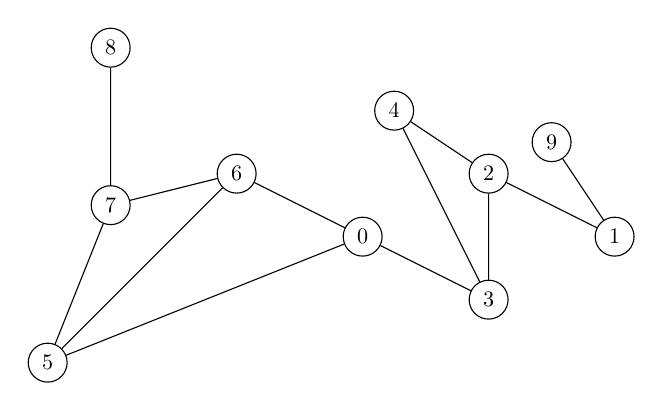
\begin{tikzpicture}[scale=0.8, transform shape]
            \node[draw,circle] (0)at(0,0) {0};
            \node[draw,circle] (1)at(4,0) {1};
            \node[draw,circle] (2)at(2,1) {2};
            \node[draw,circle] (3)at(2,-1) {3};
            \node[draw,circle] (4)at(0.5,2) {4};
            \node[draw,circle] (5)at(-5,-2) {5};
            \node[draw,circle] (6)at(-2,1) {6};
            \node[draw,circle] (7)at(-4,0.5) {7};
            \node[draw,circle] (8)at(-4,3) {8};
            \node[draw,circle] (9)at(3,1.5) {9};

            \draw[-,>=latex] (1) -- (2);
            \draw[-,>=latex] (9) -- (1);
            \draw[-,>=latex] (4) -- (2);
            \draw[-,>=latex] (7) -- (8);
            \draw[-,>=latex] (5) -- (6);
            \draw[-,>=latex] (6) -- (7);
            \draw[-,>=latex] (7) -- (5);
            \draw[-,>=latex] (6) -- (0);
            \draw[-,>=latex] (0) -- (3);
            \draw[-,>=latex] (5) -- (0);
            \draw[-,>=latex] (3) -- (2);
            \draw[-,>=latex] (3) -- (4);

        \end{tikzpicture}
    \end{center}
\begin{center}
\begin{lstlisting}[language=Python , basicstyle=\ttfamily\small, xleftmargin=0.2em, xrightmargin=0.5em]
>>> bfs_aretes(graphe)
[(0, 3), (0, 5), (0, 6), (3, 0), (3, 2), (3, 4), (5, 0), (5, 6), (5, 7), (6, 0), (6, 5), (6, 7), (2, 1), (2, 3), (2, 4), (4, 2), (4, 3), (7, 5), (7, 6), (7, 8), (1, 2), (1, 9), (8, 7), (9, 1)]
\end{lstlisting}
\captionof{code}{\centering Chaque sommet n'est enfilé qu'une seule fois. Chaque arête est parcourue deux fois (graphe non oirenté).}
\label{CODE}
\end{center}

\end{frame}
\begin{frame}[fragile]
    \frametitle{}
    \begin{center}
        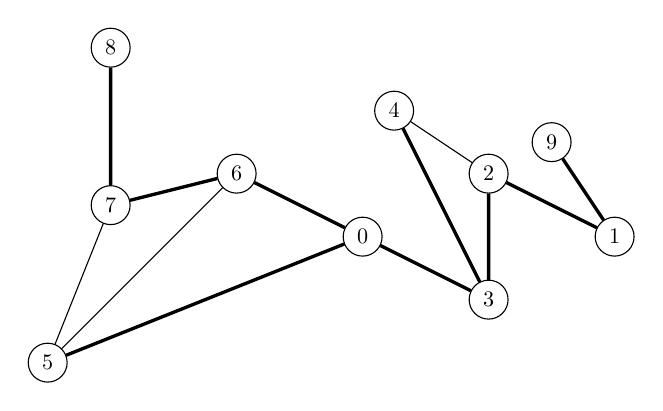
\begin{tikzpicture}[scale=0.8, transform shape]
            \node[draw,circle] (0)at(0,0) {0};
            \node[draw,circle] (1)at(4,0) {1};
            \node[draw,circle] (2)at(2,1) {2};
            \node[draw,circle] (3)at(2,-1) {3};
            \node[draw,circle] (4)at(0.5,2) {4};
            \node[draw,circle] (5)at(-5,-2) {5};
            \node[draw,circle] (6)at(-2,1) {6};
            \node[draw,circle] (7)at(-4,0.5) {7};
            \node[draw,circle] (8)at(-4,3) {8};
            \node[draw,circle] (9)at(3,1.5) {9};

            \draw[-,>=latex,very thick] (1) -- (2);
            \draw[-,>=latex,very thick] (9) -- (1);
            \draw[-,>=latex] (4) -- (2);
            \draw[-,>=latex,very thick] (7) -- (8);
            \draw[-,>=latex] (5) -- (6);
            \draw[-,>=latex,very thick] (6) -- (7);
            \draw[-,>=latex] (7) -- (5);
            \draw[-,>=latex,very thick] (6) -- (0);
            \draw[-,>=latex,very thick] (0) -- (3);
            \draw[-,>=latex,very thick] (5) -- (0);
            \draw[-,>=latex,very thick] (3) -- (2);
            \draw[-,>=latex,very thick] (3) -- (4);

        \end{tikzpicture}
    \end{center}
\begin{center}
\begin{lstlisting}[language=Python , basicstyle=\ttfamily\small, xleftmargin=2em, xrightmargin=2em]
[(0, 3), (0, 5), (0, 6), (3, 2), (3, 4), (5, 7), (2, 1), (7, 8), (1, 9)]
\end{lstlisting}
\end{center}  
\begin{aretenir}[Observation]
    Si on stocke les arêtes seulement quand on enfile les voisins, elles ne sont pas toutes visitées.
    \end{aretenir}
\end{frame}
\end{document}
